% This example An LaTeX document showing how to use the l3proj class to
% write your report. Use pdflatex and bibtex to process the file, creating 
% a PDF file as output (there is no need to use dvips when using pdflatex).

% Modified 

\documentclass{l3proj}
\begin{document}
\title{Grammar ToolKit: A Tool for Creating and Editing Grammars}
\author{Lewis Carroll \\
        Betty Davis \\
        James Dean \\
        Marilyn Monroe \\
        John Wayne}
\date{9 January 2009}
\maketitle
\begin{abstract}

The abstract goes here

\end{abstract}
\educationalconsent
\tableofcontents
%==============================================================================
\chapter{Introduction}
\label{intro}

ALICE \cite{alice} was beginning to get very tired of sitting by her sister
on the bank and of having nothing to do: once or twice she had peeped into
the book her sister was reading, but it had no pictures or conversations in
it, ``and what is the use of a book,'' thought Alice, ``without pictures or
conversations?'

So she was considering, in her own mind (as well as she could, for the hot
day made her feel very sleepy and stupid), whether the pleasure of making a
daisy-chain would be worth the trouble of getting up and picking the
daisies, when suddenly a White Rabbit with pink eyes ran close by her.

There was nothing so very remarkable in that; nor did Alice think it so
very much out of the way to hear the Rabbit say to itself ``Oh dear! Oh
dear! I shall be too late!'' (when she thought it over afterwards it
occurred to her that she ought to have wondered at this, but at the time it
all seemed quite natural); but, when the Rabbit actually took a watch out
of its waistcoat-pocket, and looked at it, and then hurried on, Alice
started to her feet, for it flashed across her mind that she had never
before seen a rabbit with either a waistcoat-pocket, or a watch to take out
of it, and burning with curiosity, she ran across the field after it, and
was just in time to see it pop down a large rabbit-hole under the hedge.

In another moment down went Alice after it, never once considering how in
the world she was to get out again.

The rabbit-hole went straight on like a tunnel for some way, and then
dipped suddenly down, so suddenly that Alice had not a moment to think
about stopping herself before she found herself falling down what seemed to
be a very deep well.

Either the well was very deep, or she fell very slowly, for she had plenty
of time as she went down to look about her, and to wonder what was going to
happen next. First, she tried to look down and make out what she was coming
to, but it was too dark to see anything: then she looked at the sides of
the well, and noticed that they were filled with cupboards and
book-shelves: here and there she saw maps and pictures hung upon pegs. She
took down ajar from one of the shelves as she passed: it was labeled
``ORANGE MARMALADE'' but to her great disappointment it was empty: she did
not like to drop the jar, for fear of killing somebody underneath, so
managed to put it into one of the cupboards as she fell past it.

``Well!'' thought Alice to herself ``After such a fall as this, I shall think
nothing of tumbling down-stairs! How brave they'll all think me at home!
Why, I wouldn't say anything about it, even if I fell off the top of the
house!'' (which was very likely true.)

Down, down, down. Would the fall never come to an end? ``I wonder how many
miles I've fallen by this time?'' she said aloud. ``I must be getting
somewhere near the centre of the earth. Let me see: that would be four
thousand miles down, I think-'' (for, you see, Alice had learnt several
things of this sort in her lessons in the school-room, and though this was
not a very good opportunity for showing off her knowledge, as there was no
one to listen to her, still it was good practice to say it over) `` yes
that's about the right distance -- but then I wonder what Latitude or
Longitude I've got to?'' (Alice had not the slightest idea what Latitude
was, or Longitude either, but she thought they were nice grand words to
say.)

Presently she began again. ``I wonder if I shall fall fight through the
earth! How funny it'll seem to come out among the people that walk with
their heads downwards! The antipathies, I think-'' (she was rather glad
there was no one listening, this time, as it didn't sound at all the right
word) ``but I shall have to ask them what the name of the country is, you
know. Please, Ma'am, is this New Zealand? Or Australia?'' (and she tried to
curtsey as she spoke- fancy, curtseying as you're falling through the air!
Do you think you could manage it?) ``And what an ignorant little girl she'll
think me for asking! No, it'll never do to ask: perhaps I shall see it
written up somewhere.''

Down, down, down. There was nothing else to do, so Alice soon began talking
again. ``Dinah'll miss me very much to-night, I should think!'' (Dinah was
the cat.) ``I hope they'll remember her saucer of milk at tea-time. Dinah,
my dear! I wish you were down here with me! There are no mice in the air,
I'm afraid, but you might catch a bat, and that's very like a mouse, you
know. But do cats eat bats, I wonder?'' And here Alice began to get rather
sleepy, and went on saying to herself, in a dreamy son of way, ``Do cats eat
bats? Do cats eat bats?'' and sometimes ``Do bats eat cats?'' for, you see, as
she couldn't answer either question, it didn't much matter which way she
put it. She felt that she was dozing off, and had just begun to dream that
she was walking hand in hand with Dinah, and was saying to her, very
earnestly, ``Now, Dinah, tell me the truth: did you ever eat a bat?'' when
suddenly, thump! thump! down she came upon a heap of sticks and dry leaves,
and the fall was over.

Alice was not a bit hurt, and she jumped up on to her feet in a moment: she
looked up, but it was all dark overhead: before her was another long
passage, and the White Rabbit was still in sight, hurrying down it. There
was not a moment to be lost: away went Alice like the wind, and was just in
time to hear it say, as it turned a comer, ``Oh my ears and whiskers, how
late it's getting!'' She was close behind it when she turned the comer, but
the Rabbit was no longer to be seen: she found herself in a long, low hall,
which was lit up by a row of lamps hanging from the roof.

There were doors all round the hall, but they were all locked; and when
Alice had been all the way down one side and up the other, trying every
door, she walked sadly down the middle, wondering how she was ever to get
out again.

Suddenly she came upon a little three-legged table, all made of solid
glass: there was nothing on it but a tiny golden key, and Alice's first
idea was that this might belong to one of the doors of the hall; but, alas!
either the locks were too large, or the key was too small, but at any rate
it would not open any of them. However, on the second time round, she came
upon a low curtain she had not noticed before, and behind it was a little
door about fifteen inches high: she tried the little golden key in the
lock, and to her great delight it fitte!d

\begin{figure}
\begin{center}
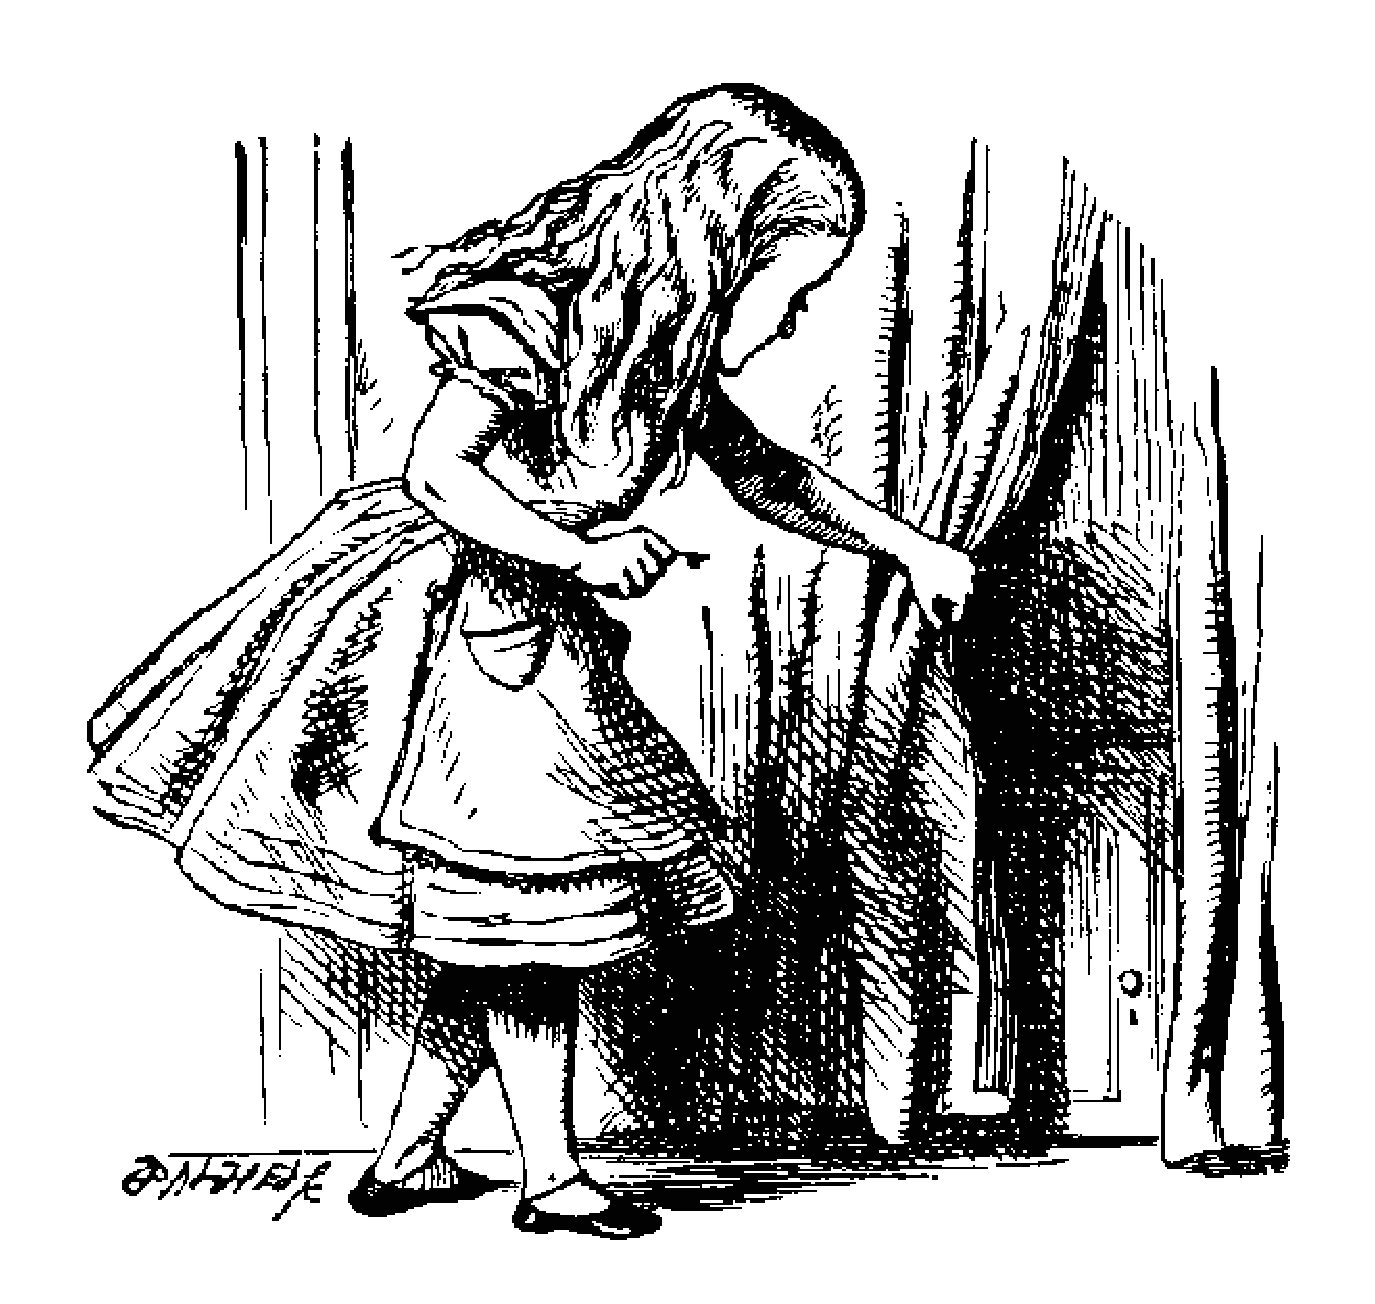
\includegraphics[width=7cm]{figures/alice}
\end{center}
\caption{Behind it was a little door}
\label{fig:alice}
\end{figure}

Alice opened the door and found that it led into a small passage, not much
larger than a rat-hole: she knelt down and looked along the passage into
the loveliest garden you ever saw. How she longed to get out of that dark
hall, and wander about among those beds of bright flowers and those cool
fountains, but she could not even get her head through the doorway; ``and
even if my head would go through,'' thought poor Alice, ``it would be of very
little use without my shoulders. Oh, how I wish I could shut up like a
telescope! I think I could, if I only knew how to begin.'' For, you see, so
many out-of-the- way things had happened lately, that Alice had begun to
think that very few things indeed were really impossible.

There seemed to be no use in waiting by the little door, so she went back
to the table, half hoping she might find another key on it, or at any rate
a book of rules for shutting people up like telescopes: this time she found
a little bottle on it, (``which certainly was not here before,'' said Alice),
and tied round the neck of the bottle was a paper label, with the words
``DRINK ME'' beautifully printed on it in large letters.It was all very well
to say ``Drink me,'' but the wise little Alice was not going to do that in a
hurry. ``No, I'll look first,'' she said, ``and see whether it's marked
'poison' or not''; for she had read several nice little stories about
children who had got burnt, and eaten up by wild beasts, and other
unpleasant things, all because they would not remember the simple rules
their friends had taught them: such as, that a red-hot poker will burn you
if you hold it too long; and that, if you cut your finger very deeply with
a knife, it usually bleeds; and she had never forgotten that, if you drink
much from a bottle marked ``poison,'' it is almost certain to disagree with
you, sooner or later.However, this bottle was not marked ``poison,'' so Alice
ventured to taste it, and, finding it very nice (it had, in fact, a sort of
mixed flavour of cherry-tart, custard, pine-apple, roast turkey, toffy, and
hot buttered toast), she very soon finished it off.

``What a curious feeling!'' said Alice. ``I must be shutting up like a
telescope!''

And so it was indeed: she was now only ten inches high, and her face
brightened up at the thought that she was now the right size for going
through the little door into that lovely garden. First, however, she waited
for a few minutes to see if she was going to shrink any further: she felt a
little nervous about this; ``for it might end, you know,'' said Alice to
herself; ``in my going out altogether, like a candle. I wonder what I should
be like then?'' And she tried to fancy what the flame of a candle looks like
after the candle is blown out, for she could not remember ever having seen
such a thing.

After a while, finding that nothing more happened, she decided on going
into the garden at once; but, alas for poor Alice! when she got to the
door, she found she had forgotten the little golden key, and when she went
back to the table for it, she found she could not possibly reach it: she
could see it quite plainly through the glass, and she tried her best to
climb up one of the legs of the table, but it was too slippery; and when
she had tired herself out with trying, the poor little thing sat down and
cried.

``Come, there's no use in crying like that!'' said Alice to herself rather
sharply. ``I advise you to leave off this minute!'' She generally gave
herself very good advice (though she very seldom followed it), and
sometimes she scolded herself so severely as to bring tears into her eyes;
and once she remembered trying to box her own ears for having cheated
herself in a game of croquet she was playing against herself, for this
curious child was very fond of pretending to be two people. ``But it's no
use now,'' thought poor Alice, ``to pretend to be two people! Why, there's
hardly enough of me left to make one respectable person!''

Soon her eye fell on a little glass box that was lying under the table: she
opened it, and found in it a very small cake, on which the words ``EAT ME''
were beautifully marked in currants. ``Well, I'll eat it,'' said Alice, ``and
if it makes me grow larger, I can reach the key; and if it makes me grow
smaller, I can creep under the door: so either way I'll get into the
garden, and I don't care which happens!''

She ate a little bit, and said anxiously to herself ``Which way? Which
way?'', holding her hand on the top of her head to feel which way it was
growing; and she was quite surprised to find that she remained the same
size. To be sure, this is what generally happens when one eats cake; but
Alice had got so much into the way of expecting nothing but out-of-the-way
things to happen, that it seemed quite dull and stupid for life to go on in
the common way.

So she set to work, and very soon finished off the cake. 

%==============================================================================
\chapter{Design}
\label{design}

The following diagrams (especially figure \ref{fig:alice}) illustrate the
process...

%==============================================================================
\chapter{Implementation}
\label{impl}

In this chapter, we describe how the implemented the system.

%------------------------------------------------------------------------------
\section{User Interface}

Blah blah blah
Blah blah blah
Blah blah blah
Blah blah blah

% - - - - - - - - - - - - - - - - - - - - - - - - - - - - - - - - - - - - - - -
\subsection{Foo}

Blah blah blah
Blah blah blah
Blah blah blah
Blah blah blah

%------------------------------------------------------------------------------
\section{Database Model}

\begin{enumerate}
\item Blah blah blah
\item Blah blah blah
\item Blah blah blah
\item Blah blah blah
\end{enumerate}



%==============================================================================
\chapter{Evaluation}

We evaluated the project by...

%==============================================================================
\chapter{Conclusion}

A great project!

%==============================================================================
\section{Contributions}

Here we explain that Lewis Carroll wrote chapter \ref{intro}. John Wayne
was out riding his horse every day and didn't do anything. Marilyn Monroe
was great at getting the requirements specification and coordinating the
writing of the report. Betty Davis did the coding of the kernel of the
project, described in Chapter \ref{impl}.  James Dean handled the
multimedia content of the project.

%==============================================================================
\bibliographystyle{plain}
\bibliography{example}
\end{document}
